\documentclass[a4]{article}
\usepackage{epsfig}
\usepackage{url}
\usepackage{color}
\newcommand{\etal}{\emph{et al.}}
\newcommand{\VH}{\mbox{V\kern-.1667em \lower.5ex\hbox{\scriptsize H}}}
\newcommand{\VL}{\mbox{V\kern-.1667em \lower.5ex\hbox{\scriptsize L}}}
\newcommand{\VHVL}{\mbox{\VH/\VL}}
\newcommand{\CH}[1]{\mbox{C\lower.5ex\hbox{\scriptsize H}#1}}
\newcommand{\CL}{\mbox{C\kern-.0833em \lower.5ex\hbox{\scriptsize L}}}
\newcommand{\FV}{\mbox{\it Fv}}
\newcommand{\Fab}{\mbox{\it Fab}}
\newcommand{\andrew}[1]{{\color{red} [*** Andrew: #1 ***]}}
\newcommand{\james}[1]{{\color{green} [*** James: #1 ***]}}
\setlength{\emergencystretch}{1in}

\let\shortcite\cite

\bibliographystyle{unsrt}

\title{A Notation Language for Bispecific Antibody Formats (Antibody
Markup Language) and Software for Obtaining Expressions for Desired
Antibodies (abYdraw)}
\author{James Sweet-Jones, Maham Ahmad, Andrew C.R. Martin\\
Institute of Structural and Molecular Biology,\\
Division of Biosciences, University College London,\\
Darwin Building, Gower Street,\\
London, WC1E 6BT, UK}

\begin{document}
\maketitle

\begin{abstract}
Multi-specific antibodies (MsAbs) are an up-and-coming class of biologic
drugs that differ from monoclonal antibodies through their ability to
bind to more than one type of antigen. As techniques to generate such
molecules have diversified, so have their formats and the need for
standard notation. Previous efforts for developing a notation language
for macromolecule drugs have been insufficient or too complex for describing
MsAbs. Here, we present Antibody Markup Language (AbML), a new
notation language specifically for antibody formats which overcomes
the limitations of existing languages and can annotate all
current MsAb formats as well as all currently conceivable future formats.
To assist users in this language we have also
developed a tool, abYdraw, that can draw antibody schematics from AbML
descriptor strings or generate a descriptor string from a drawn
antibody schematic. AbML has potential to become a standardised
notation for describing new MsAb formats entering clinical trials.
\end{abstract}

\section{Introduction}

Immunoglobulins, otherwise known as antibodies, have become useful molecular
tools in biology and medicine owing to their natural ability to bind a
specific antigen. When clonally expanded, monoclonal antibodies (mAbs)
have clinical applications spanning molecular diagnostic assays, to medical
imaging as well as therapeutics \cite{ma:2021}.
Multi-specific Antibodies (MsAbs) are engineered proteins
that differ from naturally occurring mAbs in their ability to bind to
more than one type of antigen. Generally this is achieved through multiple
different antigen combining sites and the popularity of these formats
has now been recognized by the WHO International Nonproprietary Names
(INN) which now gives the suffix stem `-mig' to such proteins
(\url{https://cdn.who.int/media/docs/default-source/international-nonproprietary-names-(inn)/new_mab_-nomenclature-_2021.pdf}).
An exception to the use of multiple combining sites is bimekizumab
which is a conventional IgG, but binds to both IL-17A and IL-17F
through a single type of combining site \cite{adams:bimekizumab}.
This would not be given the `-mig' stem in the new INN scheme.
While the majority of MsAbs are bispecific (binding to two epitopes though
different combining sites), 
trispecific and tetraspecific antibodies have also been developed.
This makes them a versatile class of molecules
which has become a keen focus of therapeutics in clinical trials
because multi-specificity allows two molecules (as is the case with emicizumab)
or two cells (as is the case with blinatumomab and catumaxomab)
to be brought into close proximity \cite{fan:2015}.
There is a particular interest in immunomodulatory cancer treatments
\cite{labrijn:2019}, in which the two currently FDA-approved
drugs mentioned above (blinatumomab and catumaxomab) are used
\cite{wilke:2017,seimetz:2011}. The only other approved MsAb (also mentioned
above) is emicizumab for Factor~VIII deficiency haemophilia \cite{schmitt:2021}. 

The engineering of these molecules has evolved over time since their
inception in the 1970s. At first, the `quadroma' was created by fusing two
hybridoma cell lines, used for generating mAbs which would then result
in some cases where two halves with different Fab fragments form
heterodimers which results in a molecule with two specificities
\cite{milstein:1983,kontermann:2015}. This
technique offered poor yield due to the disfavoured formation of the
desired heterodimers. For example, given one hybridoma
producing \VH{a}/\VL{a} and another producing \VH{b}/\VL{b}, accounting
for symmetry, 10 possible antibodies could be produced by the quadroma:
\VH{a}/\VL{a}--\VH{a}/\VL{a}, \VH{a}/\VL{a}--\VH{a}/\VL{b},
\VH{a}/\VL{a}--\VH{b}/\VL{a}, \VH{a}/\VL{b}--\VH{a}/\VL{b},
\VH{a}/\VL{b}--\VH{b}/\VL{a}, \VH{a}/\VL{b}--\VH{b}/\VL{b},
\VH{b}/\VL{a}--\VH{b}/\VL{a}, \VH{b}/\VL{a}--\VH{b}/\VL{b},
\VH{b}/\VL{b}--\VH{b}/\VL{b} and finally \VH{a}/\VL{a}--\VH{b}/\VL{b},
the desired product. Consequently efforts for more scalable synthesis have
led to new techniques of MsAb generation \cite{spiess:2015}. 

DNA recombination has allowed greater flexibility in designing MsAbs
with IgG-like formats, which can be done by appending additional Fv
fragments at the N-termini of the light and heavy chains
\cite{brinkmann:2017}. On dimerization, this approach generates a symmetrical MsAb.
Recombination also allows linking of \VH\ and \VL\ domains to
form single chain Fv (scFv) fragments
which may be sequentially added via engineered
linkers onto the N- or C-termini of both light and heavy chains.
\cite{legall:1999}. Camelid single domain VHH fragments (nanobodies)
may be added in the same way. All of these give rise to symmetrical antibodies.

Alternatively asymmetric antibodies can be produced by introducing mutations
that encourage heterodimerization of heavy chains or specific pairings of light and heavy chains.
Additional residue mutations for knobs-into-holes (KIH)
formats \cite{ridgway:1996} are typically used to form heavy chain heterodimers
by introducing mutations in \CH{3},
while introduction of positively and negatively
charged residues in the \CH{1} and \CL\ of one arm \cite{gunasekaran:2010} assist in the correct
pairing of light and heavy chains to make the desired asymmetric antibody format more favourable
\cite{spiess:2015}.   

Protein engineering also allows for generation of 
smaller fragment-based MsAbs including 2-chained diabodies or a single
chain consisting of a sequence of scFvs.
These non-IgG-like molecules are
advantageous because they are easier to produce (requiring no glycosylation),
but they are limited by short
half-lives, which can be extended through human serum albumin (HSA)
fusion or PEGylation (addition of polyethylene glycol), or the addition of
disulphide bonds \cite{kontermann:2011,ma:2021}. 

Antibody-drug-conjugates (ADCs) have become
popular methods of delivering small molecule drugs to an intended
target \cite{sau:2017}. Most recently chemical conjugation has also been exploited to allow modular combination of protein domains which
has given rise to great diversity in structures and presentation of
these molecules \cite{spiess:2015}. Ligating antibody
fragments in this was has been seen in the `Dock and Lock' format
while the potential of chemical ligation
has also been demonstrated through production of MsAbs by ligating two IgG molecules to
give IgG-IgG molecules \cite{szijj:2021}.  

While only three MsAbs have thus-far been approved (all bispecifics)
many more are in development and in clinical trials.
Given the huge diversity of possible MsAbs formats, they require a
standardized format for description and annotation when they are
submitted for an INN or for regulatory approval. For small-molecule drugs,
`Simplified Molecular-Input Line-Entry System' (SMILES) strings 
\cite{weininger:smiles} have been adopted as a standard for describing
organic molecules. As yet, no such standard has been widely adopted for biologics.

The Hierarchical Editing Language for Macromolecules (HELM) \cite{zhang:2012} was
introduced in 2012 as a general tool for describing biologics (including antibodies) and is promoted by
the Pistoia Alliance
(\url{https://www.pistoiaalliance.org/projects/current-projects/hierarchical-editing-language-for-macromolecules/}).
It provides a visual editor and has the support of a number of large pharmaceutical companies
including GlaxoSmithKline, Merck, Roche and Pfizer. 
Nonetheless, it has only gained limited traction in the annotation of antibodies
and is not currently used by regulatory authorities, the INN or the
Chemical Abstracts Service (CAS) for description of antibody-based drugs.
Current limitations which make HELM less suitable for MsAbs are (i)~its
necessary complexity (it was designed to be able to annotate any type of
complex biologic), (ii)~it does not allow for
notation of Fv fragment specificities, (iii)~it does not allow comments or notes
about additional fused domains that can be added to an antibody.
Furthermore, the HELM editor does not have specific
expressions for antibody-based drugs as it requires amino acid
sequences to draw a schematic of a molecule, which is not suitable
when describing multi-chain fragmented MsAbs.
\andrew{Is this all true still for the HELM Antibody Editor (HAbE)?
  \url{https://pistoiaalliance.atlassian.net/wiki/spaces/HELM/pages/2683306085/HELM+Antibody+Editor+HAbE}}

In this paper, we present a new antibody annotation language, Antibody
Markup Language (AbML), designed specifically to address the needs of
the antibody community in describing the ever-increasing diversity of
MsAbs in a simple and effective manner. We have also developed a
graphical editor, abYdraw, which uses AbML to render schematics of
MsAbs, as well as produces expressions from drawn antibody schematics.

\section{Methods}

\subsection{Development of Antibody Markup Language (AbML)}
The requirements for AbML were as follows:
\begin{itemize}
\item The language needed to be simple to encourage its use.
\item It needed to be sufficiently flexible to describe all current
  MsAb formats and all those that could be envisioned in future.
\item As well as standard antibody domains, it needed to be able to
  describe modified domains (e.g.\ knobs-into-holes), non-antibody
  domains and chemical conjugation.
\item Interactions between domains and (multiple) disulphides linking
  domains needed to be described.
\item The specificity of different \VHVL\ domains needed to be
  indicated.
\item Three types of connection between domains needed to be allowed:
  normal peptide connections between domains, natural (or engineered)
  hinge regions and artificial (engineered) peptide linkers.
\item AbML needed to support additional optional comments including
  general notes, types of additional domains, modifications and region
  lengths.
\end{itemize}
  
With these requirements in mind, the formats of over 60 MsAbs
described by Spiess \shortcite{spiess:2015} were used as a starting
point to ensure all such formats could be described. New INN
annotations of MsAbs (post 2016) were also examined to ensure that
they could all be annotated.

It was decided that AbML should have a similar structure to HELM
\cite{zhang:2012}, but simplified and adapted specifically for MsAbs.
For example, HELM would require one to
to specify a constant heavy (\verb|`CH'|) domain and add a
comment to specify which \CH\ type it is (\CH{1}, \CH{2}, etc.)
To simplify this, AbML adopts separate domain types (\verb|`CH1'|,
\verb|`CH2'|, etc.)

To improve the description of antibodies, it was decided to provide
three types of peptide connectors between domains: (i)~natural short
peptide connectors between domains (as seen, for example, joining \VH\
and \CH1\ domains). The standard definitions of the boundaries of
antibody domains include these linking peptides and consequently they
do not need to be indicated as separate regions of the structure;
(ii)~natural hinge regions (as seen between \CH1\ and \CH2\ domains);
(iii)~engineered linkers (e.g.\ between the \VH\ and \VL\ domains of
an scFv). Hinges and engineered linkers \andrew{Is this true for
  linkers in abYdraw?} differ from natural connectors in that they can
be considered as connector-based `domains' that can interact with one
another and be joined via disulphide bonds.

\subsection{Development of abYdraw}
abYdraw was initially developed to render AbML strings as images, but
was then extended to make AbML more accessible by providing a
graphical editor. abYdraw allows an AbML string to be entered via
the graphical user interface and rendered as an image or an image can
be created or manipulated to generate an AbML string.
abYdraw was implemented in Python3 using TKinter (a standard Python
package) for the interface.


\begin{figure}
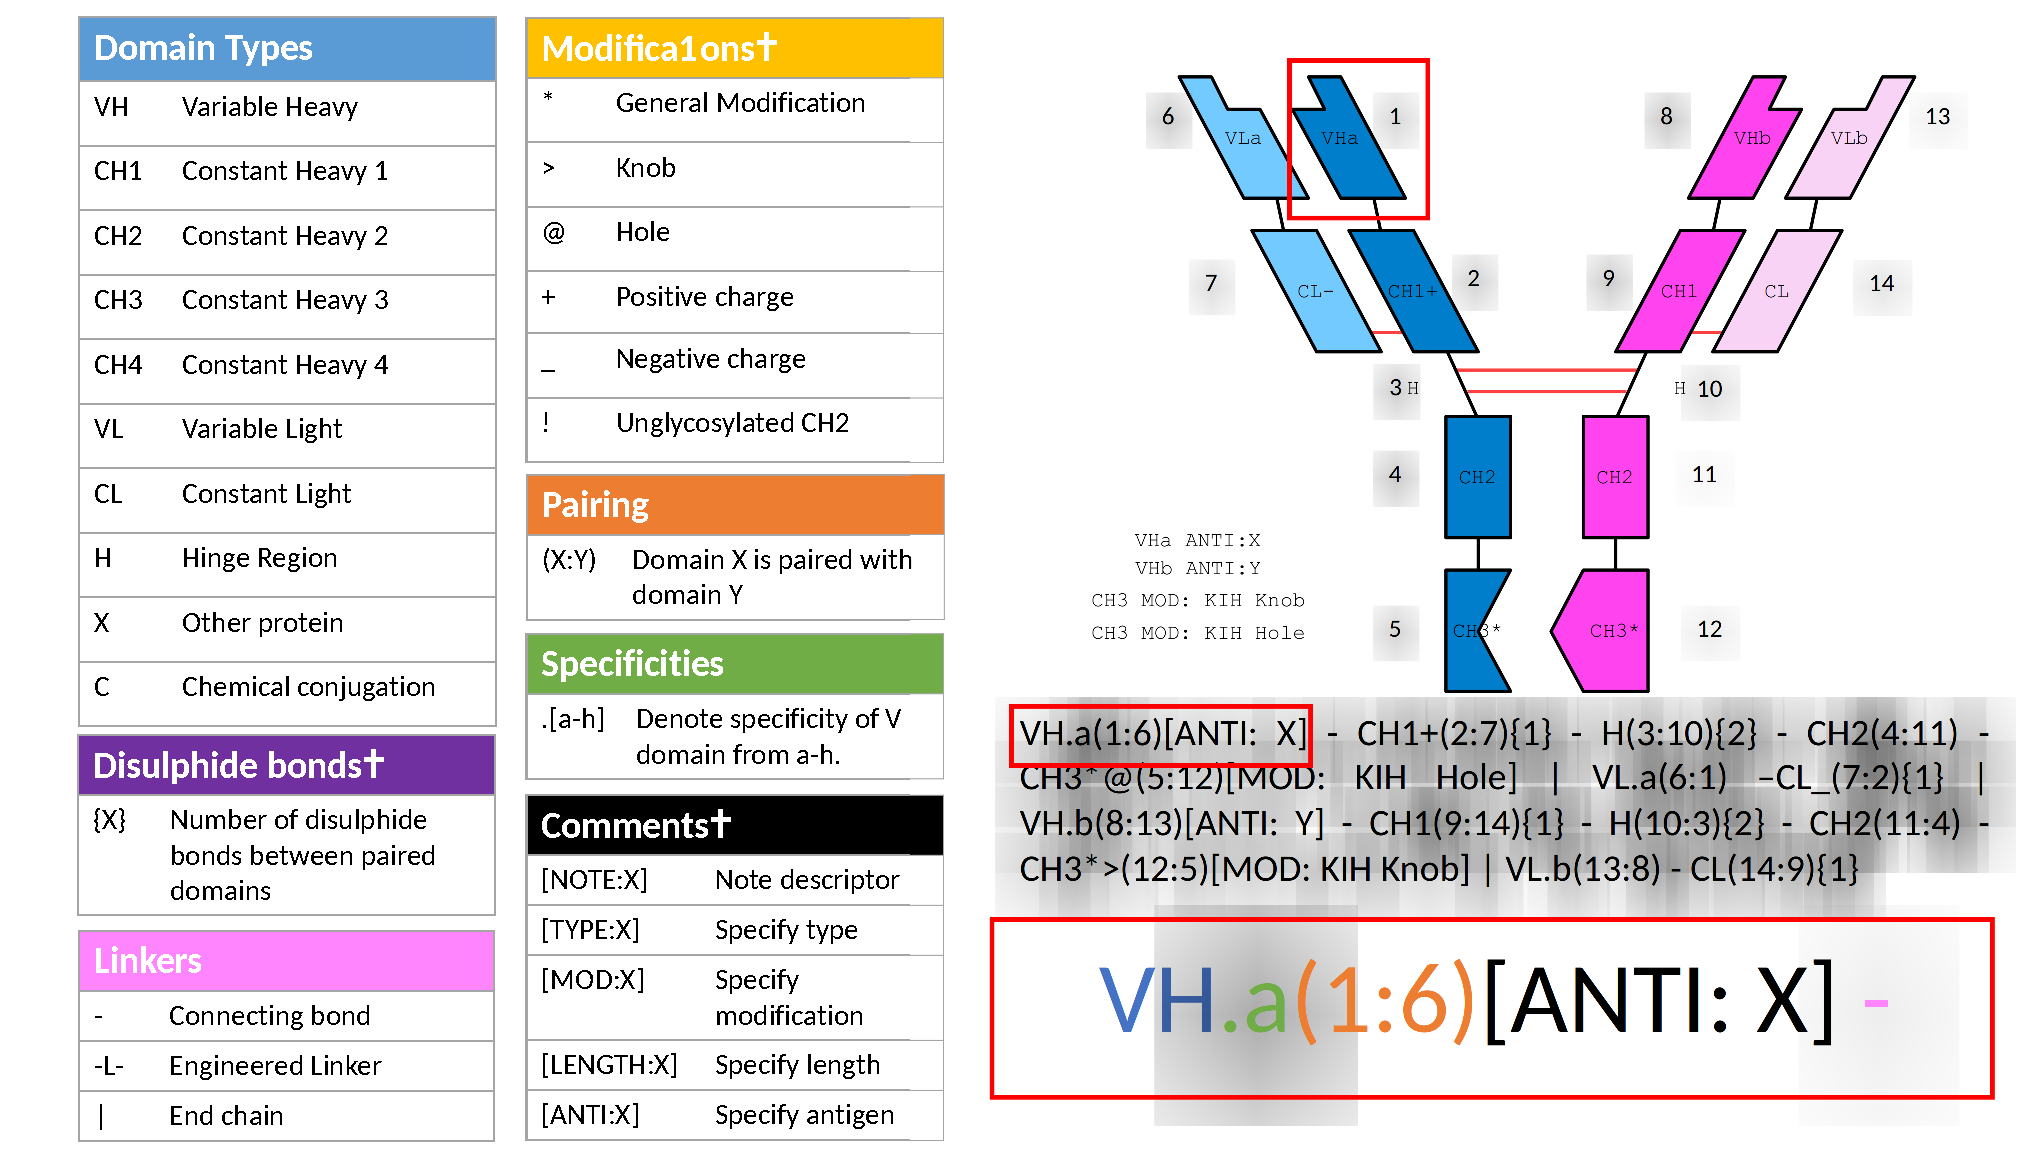
\psfig{width=\columnwidth,file=Figure1.eps}
\caption{\label{fig:1} AbML Guidesheet Explaining the Properties of
the Language. All possible domain types, modifications, connectors and
comment types as well as how to notate pairings and disulphide bonds
are given in colour-coded fashion to the example antibody domain
highlighted in red. Antibody schematic was rendered with abYdraw and
numbers represent the numbering of each domain given in AbML and
labelled on the schematic. \andrew{What does the dagger mean next
  to Disulphide Bonds and Comments? As I remember there are some
  TYPEs with special meaning - e.g.\ leucine zipper. I don't think
  we currently have anything to indicate specific ADC sites (many
  ADCs are just conjugated via any available lysines, but that is
  changing. Should `Engineered Linker' come under Domains? (Since
  Hinge does?). The hinge colour doesn't match what it says in the
  text. I suggest a section title of `Connectors' rather than
  `Linkers'}}
\end{figure}

\section{Results}

\subsection{Antibody Markup Language}
AbML is based on describing antibody domains, arranged in a string and
separated by connectors, representing a chain from an antibody
from N-terminus to C-terminus. The aim is to provide as simple a format
as possible while conveying all necessary information.

Each domain is separated by a
\verb|`-'| character and is numbered sequentially in
order of its appearance in the expression. 
In this respect, hinges and artificial linkers can be considered more
like domains as they are numbered and are separated from neighbouring
domains with a \verb|`-'| character.
Whitespace, including line breaks are ignored in AbML
except for comments given in square braces.

Chains are separated by \verb.`|'.
characters. Chains that are part of the antibody molecule can be
presented in any order, but any additional chains that interact with it
(e.g.\ via a disulphide or a domain pairing with a domain conjugated to the antibody)
are placed last. In a multi-chain structure, every chain must have at least one domain
that interacts with a domain on a different chain.

\subsubsection{Domains}
A domain annotation always begins with the domain type.
The following domain types are permitted: 
\verb|`VH'|, \verb|`VL'|,
\verb|`CH1'|, \verb|`CH2'|, \verb|`CH3'|, \verb|`CH4'|, \verb|`CL'|,
\verb|`X'|, \verb|`C'|, \verb|`H'| and \verb|`L'|] as explained in the
language guide sheet (Figure~\ref{fig:1}). 
\verb|`X'| domains are `extra' domains that are not part of a
standard immunoglobulin and will usually be described by associated comments;
\verb|`C'| domains are chemical conjugation moieties, while \verb|`H'|
and \verb|`L'| refer to hinge regions and artificial linkers respectively.

For the Fv fragment, (i.e.\ \VH\ and \VL\ domains, the specificity is
indicated by appending a \verb|`.'| followed by a letter corresponding
to the specificity (e.g.\ \verb|VH.a|)  \andrew{abYdraw requires this
  is always specified. For single specificity antibodies, it would be
  good if it weren't needed.}

Where a \VHVL\ can bind multiple antigens (as is the case with
bimekizumab, as noted above), this can be indicated with multiple
letters (e.g.\ \verb|VH.ab|, \verb|VL.ab|).
Typically, an interacting pair of \VH\ and \VL\ domains
would both be assigned identical specificity descriptors, but
exceptions apply when two different heavy chains share a common light
chain.
In this case one heavy chain would be \verb|VH.a| and the other would
be \verb|VH.b|, while the light chain would be \verb|VL.ab|).
\andrew{Have I understood this correctly?}.


Each domain is given a unique identifying number in parentheses (e.g.\
\verb|`VH.a(1)'|) and this notation can be extended to indicate a domain
with which it interacts by following the domain number with a colon
and the identifying number of another domain (e.g.\
\verb|`VH.a(1:6)'|).

If the interacting domains have disulphide bonds between them, these
are indicated in curly brackets to indicate
the number of disulphide bonds. (e.g.\ \verb|`CH1(2:7){1}'|).

Thus a normal IgG antibody could be described by the AbML string:
\begin{verbatim}
VH.a(1:6)-CH1(2:7){1}-H(3:10){2}-CH2(4:11)-CH3(5:12)|
VL.a(6:1)-CL(7:2){1}|
VH.a(8:13)-CH1(9:14){1}-H(10:3){2}-CH2(11:4)-CH3(12:5)|
VL.a(13:8)-CL(14:9){1}
\end{verbatim}

\subsubsection{Modifications}
Modifications to domains are indicated by characters immediately following the
domain type. Six such characters are currently supported.
\verb|`>'| and \verb|`@'| are used to indicate
knobs and holes respectively for knobs-into-holes heterodimer pairing.
\verb|`+'| and \verb|`_'| are used to indicate
positive or negative mutations for charge pairing. Note that
\verb|`_'| is used instead of \verb|`-'| for a negative charge since
\verb|`-'| is used between domains.

Other general modifications (e.g.\ mutations to enhance or abrogate
effector functions) can be indicated with a \verb|`*'| which can be
elaborated by a comment. Finally \verb|`!'| can only appear in \CH{2}
as it specifies that this domain is not glycosylated.

If there are multiple modification symbols, they can appear in any
order.  However, \verb|`@'| cannot be combined with \verb|`>'|, and
\verb|`+'| cannot be combined with \verb|`_'| since they are mutually
exclusive opposite modifications.

Each domain may be followed by an optional comma-separated list of comments
within a set of square brackets. These comments can denote the nature of
`extra' non-antibody protein domains as well as antigen
specificities or the length of a domain or linker. A full list of
keywords and modifications can be found on the AbML descriptor sheet
(Figure~\ref{fig:1}).

\subsection{abYdraw}
abYdraw is a graphical program written in Python3 where users may
input expressions in AbML to obtain a schematic of their designed
antibody by clicking the \verb|`Get Structure'| button. However, the user is
also able to draw antibodies by arranging standard antibody domains
and connecting them with connectors to obtain the appropriate expression
for their design by using the \verb|`Get Sequence'|
\andrew{I suggest changing to `Get AbML'} button. Once the AbML
is obtained for the drawing, using \verb|`Get Structure'| will re-render the
schematic automatically. Both functions can be run in sequence using the
\verb|`Tidy'| button. The programme will also print out comments made in the
AbML string and highlight the domain linked to those comments. abYdraw
can be used to export these schematics as figures for
publication and to generate a standardised expression that may be used
in MsAb annotations.  

The interface draws domains as blocks labelled with their domain type
and any specified modifications.  In the case of the negative charge
modification, the \verb|`_'| is replaced with a minus sign in the
rendered image.  For knobs-into-holes modifications, the \verb|`@'|
and \verb|`>'| characters are omitted as these modifications are used
to affect the shape of the rendered domain.

By default, domains are coloured according
to their specificities descriptor. It is possible that chains will
have blocks of different colours when domains of different
specificities are given in the same chain.
Normal connections between each domain are given by black lines that
are drawn from the bottom of one domain to the top of the next
domain. Artificial linkers are shown as purple lines, disulphide bonds
are shown as red lines and hinges are shown in dark green. Default
colours for all domain and bond types 
may be changed in the settings menu.


Variable domains appear
with a cut-out at the top of the domain referring to its
antigen-interacting site which pairs with another to give a complete
Fv fragment. Nanobody domains (i.e.\ a \VH\ domain that doesn't interact with
anything else) have a unique domain shape reflecting their single-domain
binding site. Knobs-into-holes adaptations are displayed by constant
domains with either a cut-out or an extension to their side which
slots together to demonstrate how these domains are paired.
\andrew{We could change the unpaired \VH\ to be called VHH instead ---
  that is used quite often for Camelid single \VH\ antibodies.}

Users may draw MsAbs from scratch or begin with a template design of
common MsAb formats that may be manipulated by the user. To draw
domains, a user must select a specificity and any modifications for that domain
and then place it on the canvas. Both specificities and modifications
can be updated whilst on the canvas by selecting a specificity or
modification, but not a domain type. Once drawn, domains may be
moved to a space where they interact with other domains to be
paired. \VH\ and \VL\ domains must face each other to be considered as
interacting. Users can right-click newly drawn domains to change the
direction they are facing. Nanobodies cannot be paired with other
domains as these are single-domain VHH fragments. Bonds connecting
domains are drawn by starting on the N-terminal domain of the pair and ending on
the C-terminal domain of the pair. Disulphide bonds can be drawn starting from either
of the interacting domains. To insert a comment, the required
comment type is selected, the comment text is typed into the
text entry box and the required domain is clicked to associate the
comment with that domain.  Clicking the \verb|`Tidy'| button will then
relocate the comment to the bottom of the canvas.

Any
comments given in the expression are printed with the domain symbol for
the domain to which it applies. If multiple comments are
given for a domain, they are printed on the same line. 

\begin{figure}
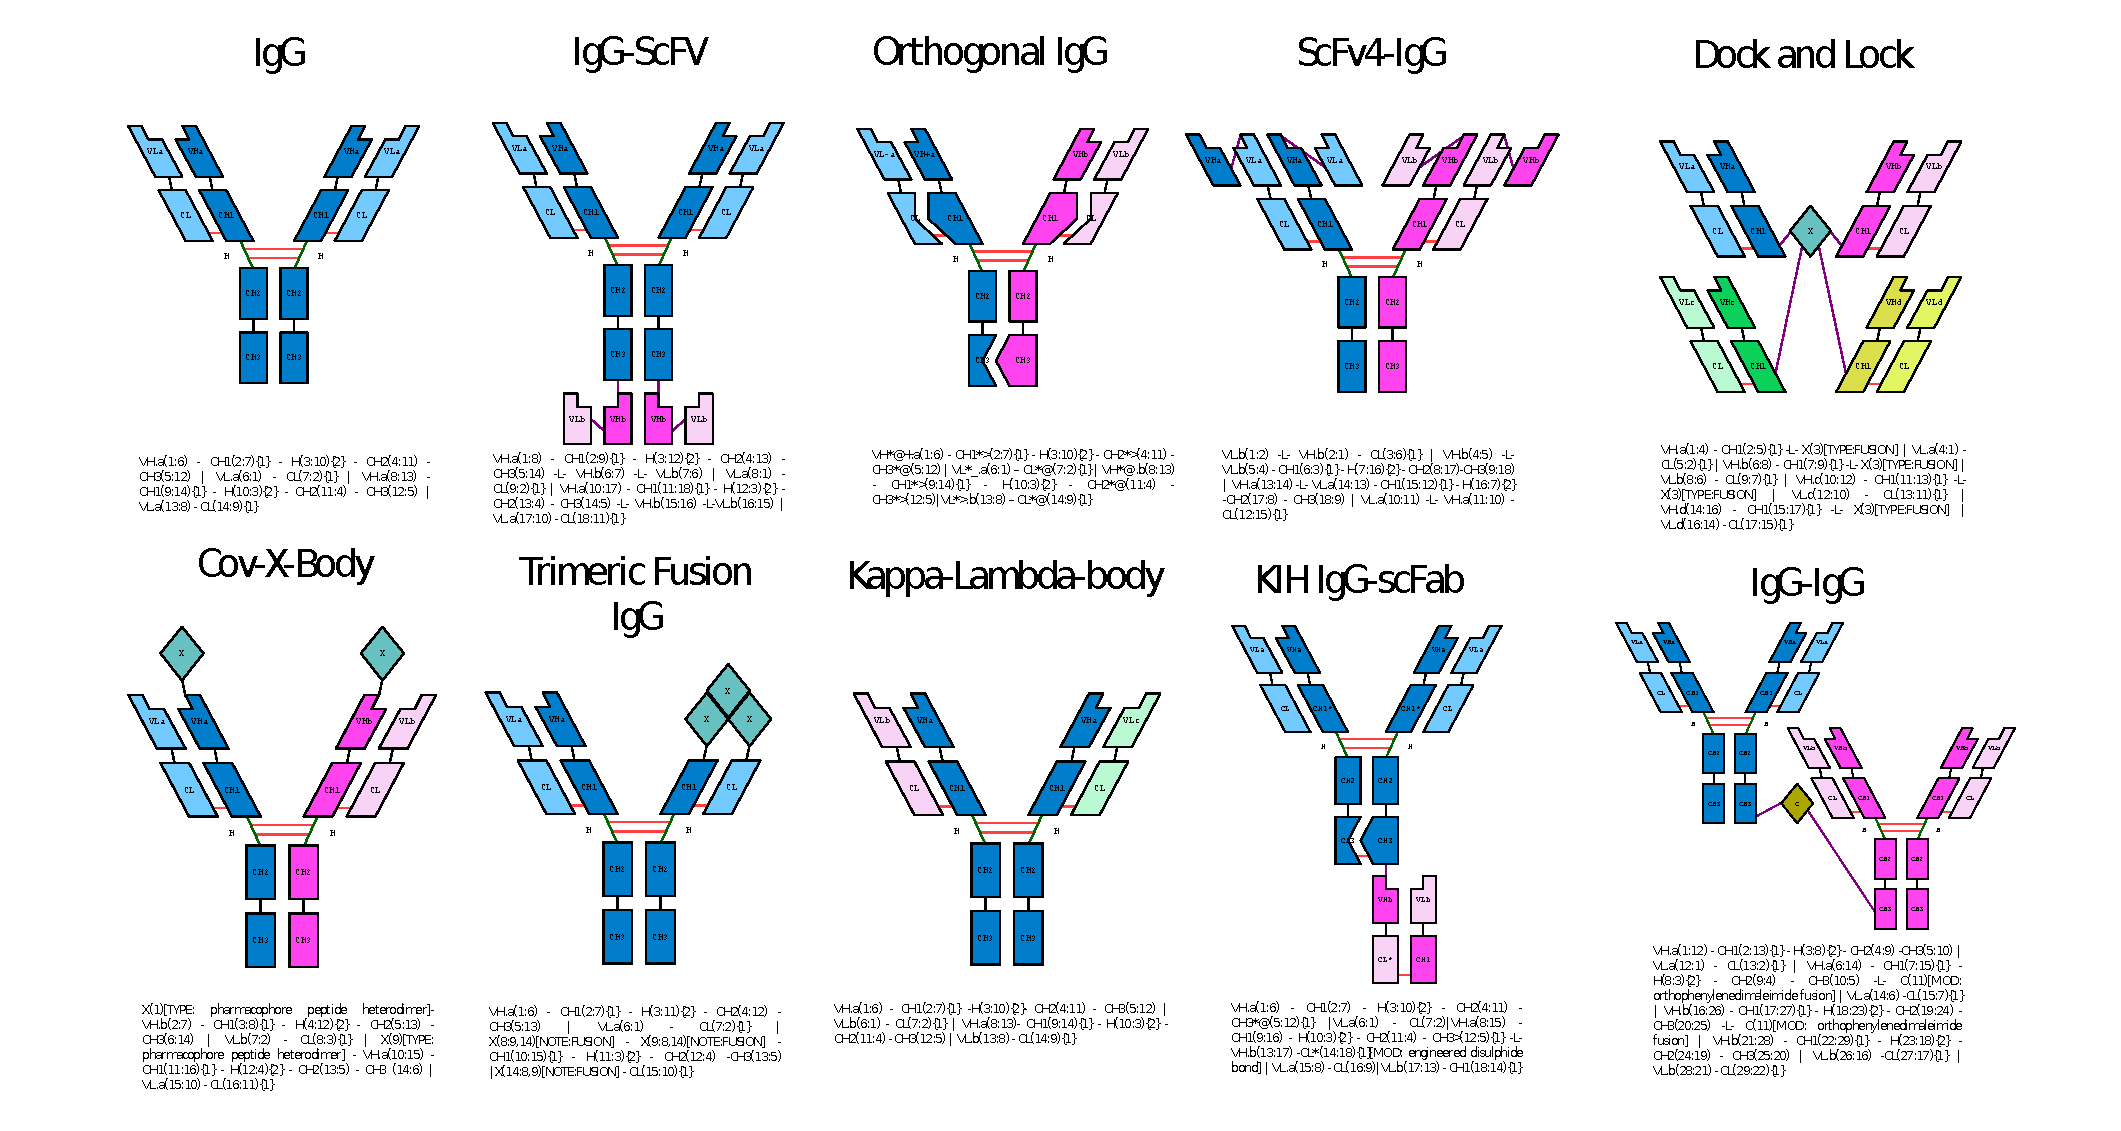
\psfig{width=\columnwidth,file=Figure2.eps}
\caption{\label{fig:2} AbML descriptor strings of commonly-used
4-chain bispecific antibodies. Schematics of antibodies were rendered
in abYdraw. \andrew{It might be better to put the AbML in supplementary
  material as it is too small to read!} }
\end{figure}

\begin{figure}
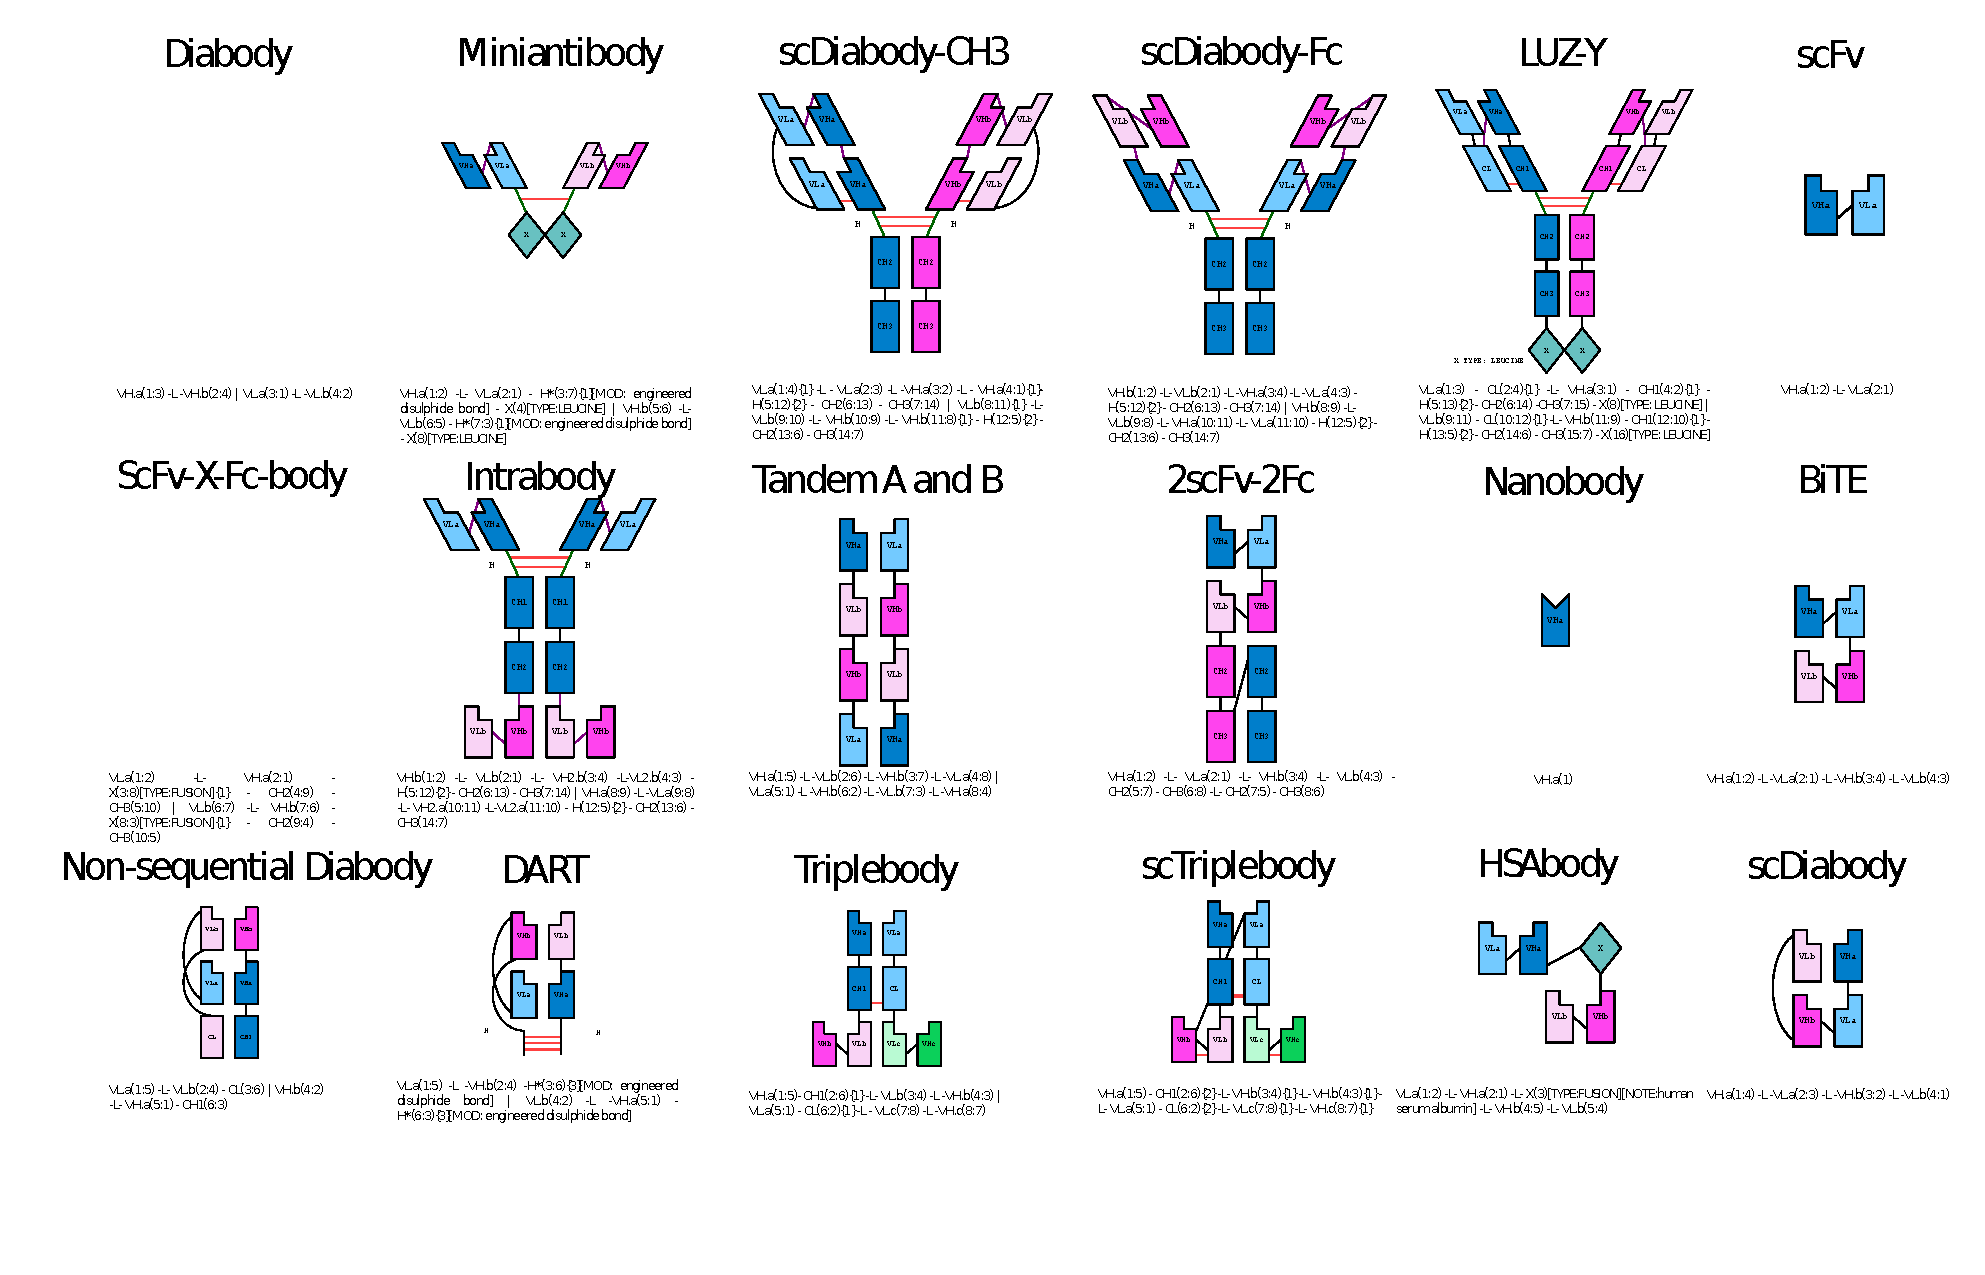
\psfig{width=\columnwidth,file=Figure3.eps}
\caption{\label{fig:3} AbML descriptor strings of commonly-used
2-chain and 1-chain bispecific antibodies. Schematics of antibodies
were rendered in abYdraw.} 
\end{figure}

Figures~\ref{fig:2} and~\ref{fig:3} demonstrate that AbML may be
applied to numerous antibody formats described by Spiess \etal
\shortcite{spiess:2015} and then rendered using abYdraw.

\section{Discussion}

By addressing the pitfalls of currently available annotation languages,
we have developed AbML which is loosely 
based on the established HELM notation for macromolecule
biologics, but simplified and adapted specifically to describe antibody
formats in a straightforward  manner.
AbML has been carefully designed to allow annotation of future possible
formats and we have demonstrated that it can be applied to all existing
MsAbs described by Spiess \etal \shortcite{spiess:2015} as well as
newer antibodies annotated by the INN.

The simplicity of AbML over HELM allows greater accessibility
as well as allowing the potential to extend the language in future by inserting additional modification
symbols and domain types that will future-proof the language to cope
with the inevitably expanding formats of recombinant and chemically
conjugated MsAbs. In general the \verb|`X'| and \verb|`C'|
domains can be used to describe a multitude of possible fusion proteins,
drug conjugates and chemical bonds using the comments system, and consequently
we do not expect the language to require constant updating.

We hope that abYdraw, which is able both to generate and render AbML,
will make AbML more accessible and will promote its use as a standard
methods for describing antibody formats.  We are also providing
compiled application versions for Mac~OS and Windows environments
avoiding the need to install Python and required libraries, and to run
the program from the command line.

abYdraw includes a library of commonly used MsAb formats complete with their AbML
strings and diagrams that can be used as starting points for
researchers to draw and describe newly designed drugs.

Currently, abYdraw has some minor limitations and is anticipated that
these may need to be addressed in future. It only supports eight
specificities (i.e.\ letters a--h), but this should be enough for all
conceivable constructs for the foreseeable future.  abYdraw also
limits domain pairings to those normally seen. i.e.\ \VHVL,
\CH{1}/\CL, \CH{2}/\CH{2}, \CH{3}/\CH{3}, \CH{4}/\CH{4}\ and
hinge-hinge. In addition interactions may be specified between `extra'
(non-antibody) domains and chemical conjugation moieties.  \andrew{Can
  it do L--L, X--C, X--L, C--L? Can it do X and/or C with any of the
  antibody domains (e.g.\ with a disulphide)}

Further developments to promote its use include adding a command-line
interface that would allow it to be used for automatically rendering
AbML strings without use of the graphical user interface. This would
be useful, for example, in the context of web pages. In future,
porting abYdraw to JavaScript would allow the full graphical user
interface to be used via a web page with no need to install software
locally.


\section{Conclusion}

To conclude, our annotation language AbML is a new descriptor language
for MsAb formats and its ability to annotate all existing MsAb formats
has been demonstrated. We expect this language and its corresponding
tool abYdraw to become useful in the development of future MsAb drugs,
allowing for standardisation of MsAb description as part of ushering
in a new era of MsAb development. Improved descriptions of their
formats will demonstrate the most popular formats and those which are
most likely to work as drugs, therefore prompting greater development
in the bispecific field.  

\section{Software Availability}
Compiled apps for Mac~OS and Windows are made free to download at:
\url{http://www.bioinf.org.uk/software/abydraw/}
Source code for this project is also made available at
\url{https://github.com/JamesSweetJones/abYdraw}

\bibliography{abYdraw} 

\end{document}
